\documentclass[border=10pt]{standalone}
\usepackage{tikz}\usepackage{amsmath}\usetikzlibrary{arrows.meta}
\begin{document}
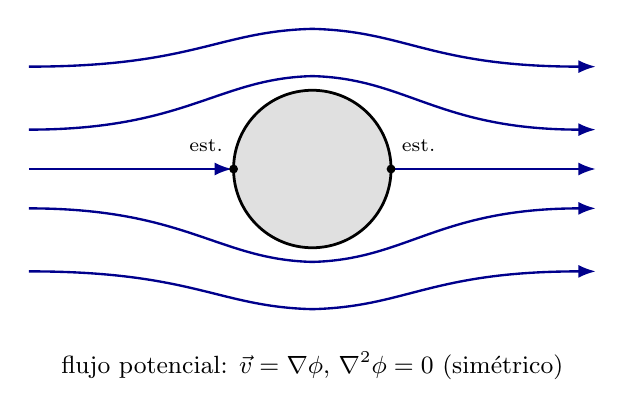
\begin{tikzpicture}[line width=0.85pt,>={Latex[length=2.2mm]}]
  \fill[black!12] (0,0) circle(1);
  \draw[line width=1pt] (0,0) circle(1);
  % lineas de corriente simetricas que rodean el cilindro
  \foreach \s in {1,-1}{
    \draw[blue!55!black,->] (-3.6,\s*0.5) .. controls (-1.6,\s*0.5) and (-1.2,\s*1.15) .. (0,\s*1.18) .. controls (1.2,\s*1.15) and (1.6,\s*0.5) .. (3.6,\s*0.5);
    \draw[blue!55!black,->] (-3.6,\s*1.3) .. controls (-1.5,\s*1.3) and (-1.2,\s*1.75) .. (0,\s*1.78) .. controls (1.2,\s*1.75) and (1.5,\s*1.3) .. (3.6,\s*1.3);
  }
  % linea central (estancamiento)
  \draw[blue!55!black,->] (-3.6,0)--(-1.02,0); \draw[blue!55!black,->] (1.02,0)--(3.6,0);
  \fill (-1,0) circle(1.6pt); \fill (1,0) circle(1.6pt);
  \node at (-1.35,0.3){\scriptsize est.}; \node at (1.35,0.3){\scriptsize est.};
  \node at (0,-2.5){\small flujo potencial: $\vec v=\nabla\phi$, $\nabla^2\phi=0$ (simétrico)};
\end{tikzpicture}
\end{document}
